{\textbf{1. 二叉排序树定义}}

{二叉排序树或者是空树,或者是满足如下性质的二叉树:}

{~(1)若它的左子树不为空,则左子树上所有关键字的值均小于根关键字的值。}

{~(2)若它的右子树不为空,则右子树上所有关键字的值均大于根关键字的值。}

{~(3)左右子树均为一棵二叉排序树。}

{如果输出二叉排序树的中序遍历序列,则它这个序列是递增有序的。}

{\textbf{2. 查找关键字}}

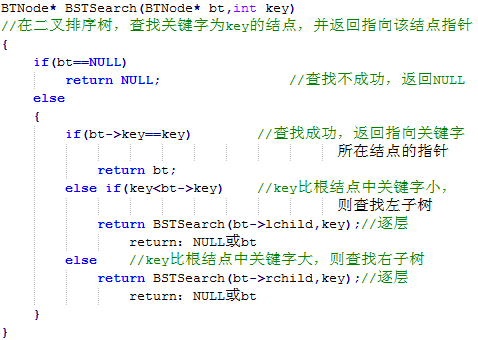
\includegraphics[width=3.70833in,height=2.63542in]{png-jpeg-pics/8CE04083F835D119A23665EED821C55A.png}

{\textbf{3. 插入关键字}}

{对查找关键字的算法进行修改即能完成插入关键字的算法。}

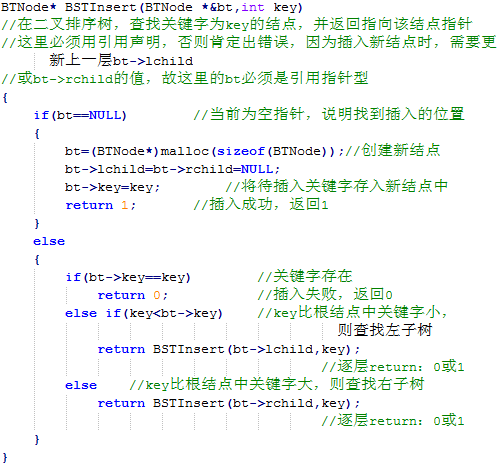
\includegraphics[width=3.70833in,height=3.43750in]{png-jpeg-pics/EAFA52E772727C988A107FA033D79A31.png}

{\textbf{4. 删除关键字}}

{假设在二叉排序树上被删除结点为p,f为其双亲结点,则删除结点p的过程分为3种情况:}

{(1)若p结点为叶子结点,直接删除即可。}

{(2)若p结点只有右子树而无左子树,或者只有左子树而无右子树。只需把p删掉,将p的子树直接连接在原来p与其双亲结点f相连的指针上即可。}

{(3)若p结点既有左子树又有右子树。}

{沿p的左子树根结点的右指针一直往右,直到右子树的最右边的结点r。将p的关键字用r中的关键字代替。最后判断,如果r是叶子结点按1)方法删除,若r是非叶子结点,则按2)方法删除r。}
